\section{Introduction}

The Republic of South Africa (RSA), often considered as the \textit{Powerhouse of Africa}, is facing many power outages or shortages of energy mainly due to the lack of investment in power infrastructure [add source from worddoc]. The RSA government is embarking on various energy and efficiency initiatives with a focus on off-grid solutions and renewable energy. The country aspires to raise an industrial revolution to shift towards a \textit{Green Economy} with the intent of boosting its manufacturing industry. This has attracted many large investors in the renewable energy sector, with the likes of Google funding Africa’s largest solar farm project in South Africa.
\vspace{5mm}\\
Furthermore, the country’s ample wind resource, especially in the Western Cape and Eastern Cape regions, as seen in Figure 1 below, make it a suitable market location for the wind energy industry. Several large scale wind farms have been installed, are under construction or have been planned since 2014. The creation of the South African wind energy industry creates a market for wind turbines that are suitable for this area. The wind turbine designed and presented in this report will therefore be made suitable for the South African onshore wind energy market.
\vspace{5mm}\\
Most wind farms in the RSA use turbines rated between 1 and 3 MW with the most recent projects leaning towards using larger turbines of at least 2 MW. Some recent projects include:
\begin{itemize}
    \item the Dorper WF Wind Farm, with 40 Nordex N100 Turbines rated at 2.5 MW
    \item the Dassiesklip Wind Farm, with 9 Sinovel SL3000 turbines rated at 3 MW (under construction)
    \item the Grassridge Wind Farm, with 20 Vestas V112 turbines rated at 3 MW, online since June 2015
\end{itemize}
 Considering the currently employed turbines in South Africa, the new design of turbine for this market will be adjusted so as to obtain the best economic performance; although, it is expected to fall in the power rating range of the abovementioned turbines.\\
 \begin{center}
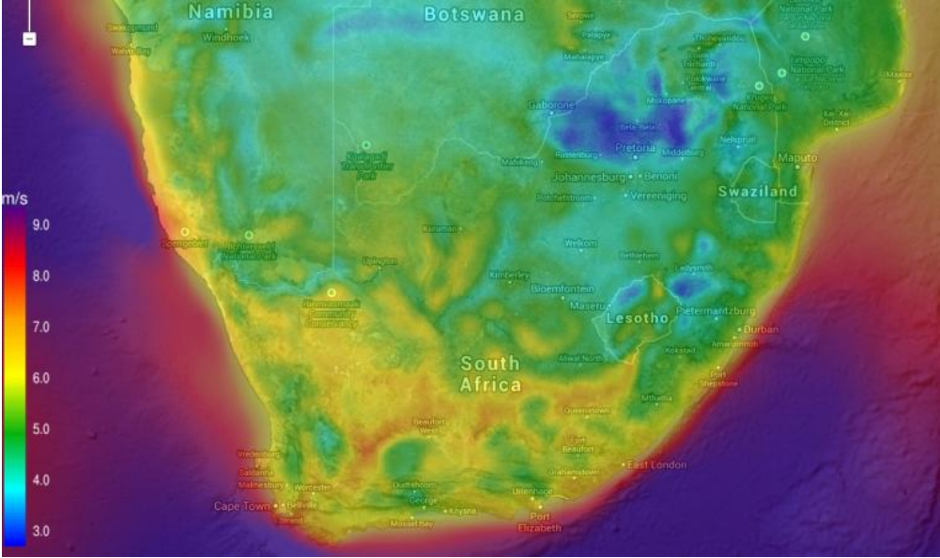
\includegraphics[width=9cm]{Images/windafrica.png}\\
Figure 1. Wind resource in South Africa [www.vortex.es]
\end{center}
\textcolor{red}{Energy price in South Africa(Although the fifth bid window will have a maximum price of 0.76 zar/kWh , the last
bid window had an average energy price of 0.619 zar/kWh (0.034 e/kWh)***(Cite:Deparment of Energy, "REIPPPP: Bid Window 4 - Preferred Bidders' Announcement",
South Africa, 2015.)***.), info about where current development already exists (location)***majority of wind turbines are located in the western and eastern cape regions as they have good wind resource***, the price of an offshore project (government support to be possible)****On average, the expected investment costs for a new offshore wind farm are currently in the range of 2.0 to 2.2 million €/MW.Cite(http://www.wind-energy-the-facts.org/development-of-the-cost-of-offshore-wind-power-up-to-2015.html)****, the specifications of the location we've chosen, the specification of the location where the wind has been measured, present the 5 MW reference turbine}